\section{Rétrospection}
\label{hindsight}

\subsection{Travail inachevé}

Si j'avais pu continuer à travailler sur le compilateur PhaistOS, je pense qu'un grand nombre d'améliorations auraient pu lui être apportées. Cependant le temps et la priorité des tâches ont fait que certains objectifs fixés pendant le stage non pas pu être réalisés. Voici une liste non-exhaustive de ces idées d'améliorations qu'on aurait bien aimé implémenter avec Nicolas :

\begin{enumerate}
    \item Créer un dossier de test avec plusieurs politiques pour pousser les analyseurs dans leur retranchement, testant ainsi leur robustesse.
    \item Créer une preuve de concept visant à montrer que le visiteur de modèle et la création d'un visiteur pour l'AST n'étaient pas nécessaire; et que l'on pouvait remplacer ces visiteurs à l'aide d'une bibliothèque~\cite{visitors2021manual}, déléguant ainsi une grande charge de travail.
    \item Régler tout les soucis de compilation ocaml présent dans les différents dossier, comme cela a été fait avec \texttt{Static-Analysis}.
    \item Créer de nouvelles politiques avec PhaistOS, basées sur celles qui existent déjà, pour pouvoir tester les limites du DSL plus en profondeur, et explorer les nouvelles pistes d'améliorations.
    \item Changer le code du point d'entrée des programmes ocaml pour offrir une interface en ligne de commande complète (\texttt{--help}, \texttt{-o}, etc.).
    \item Étendre la batterie de tests de performances avec d'autres outils, comme NAS, Phoronix, Parsec, Sysbench, etc.
\end{enumerate}

Cependant, ce n'est pas la priorité du chercheur de rendre le code plus qualitif ou robuste. Par contre, toutes ces idées pourraient faire l'objet d'un futur stage, facilitant ainsi le travail du chercheur sur la partie importante du projet de recherche. 

\subsection{Gestion de projet}

Au début du stage je n'avais pas accès aux locaux du bâtiment d'accueil, je travaillais donc depuis chez moi. Je passais des appels avec mon tuteur sur la plateforme bbb de l'UGA et on discutait de l'environement de travail et des premières tâches à réalisées. L'outil Slack nous aura aussi bien aidé pour apporter une aide à l'écrit, des fois nécessaire quand on veut partager du texte.

Les tâches principales étaient déjà définies mais restaient larges (Etude de l'existant, améliorations du compilateur, tests de performances), je les ai donc sous-divisées. J'ai adapté mes travaux au fur et à mesure, et pour illustrer ça, on peut comparer le planning de travail estimé au réel à travers les Figure~\ref{fig:gantt_1}~et~\ref{fig:gantt_2}.

\begin{figure}[h!t] \centering
    %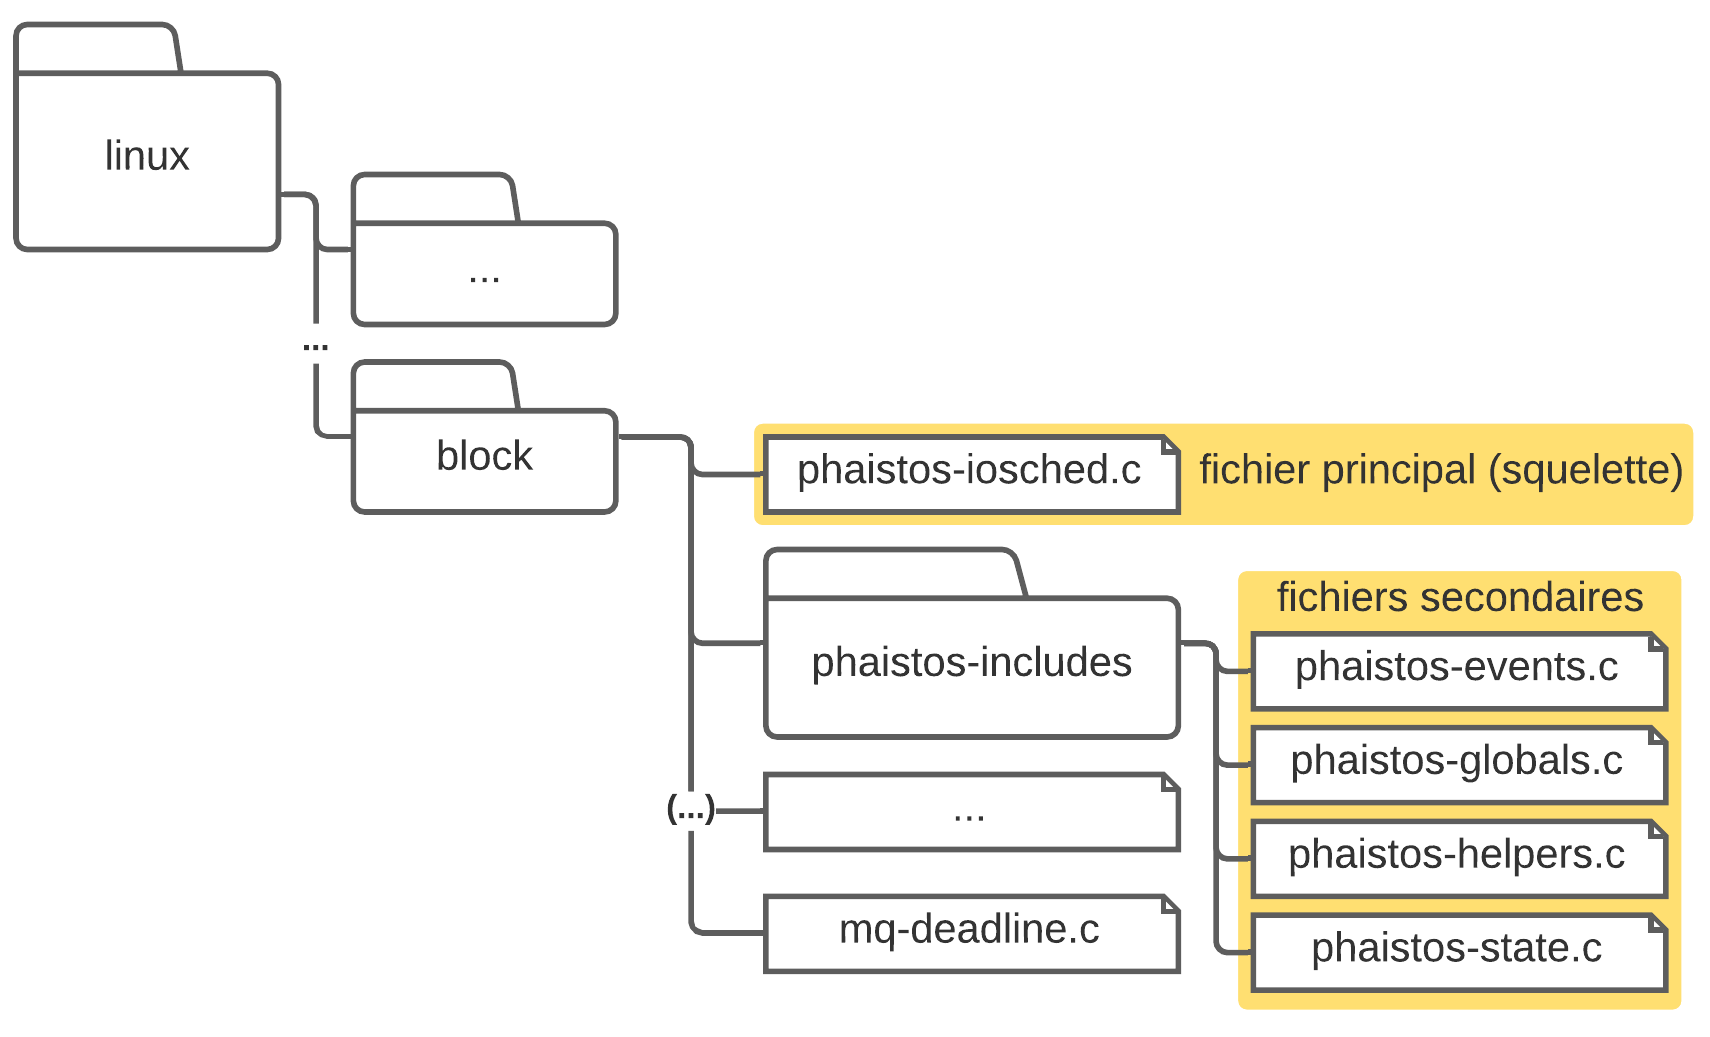
\includegraphics[width=0.8\textwidth]{images/linux_arch}
    \caption{gantt 1}
    \label{fig:gantt_1}
\end{figure}

\begin{figure}[h!t] \centering
    %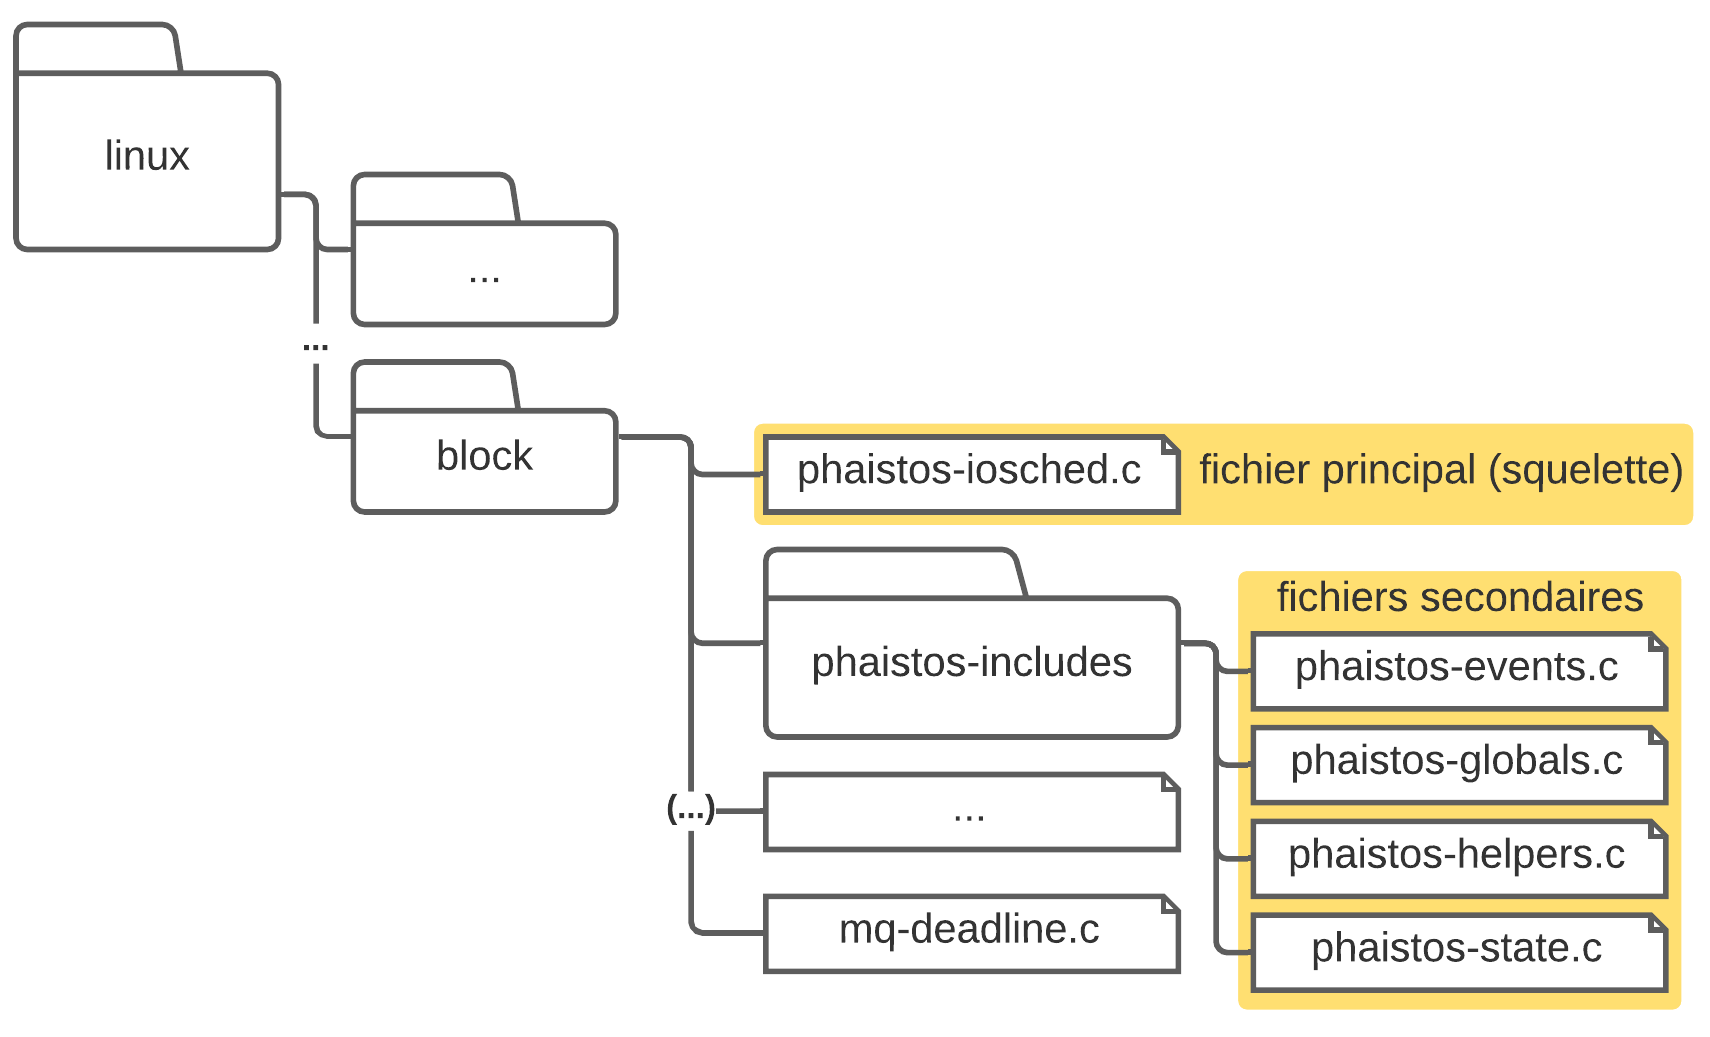
\includegraphics[width=0.8\textwidth]{images/linux_arch}
    \caption{gantt 2}
    \label{fig:gantt_2}
\end{figure}

<RETOUR SUR LES GANTT>

Il est à noter qu'à partir du 1er juillet, je pouvais me rendre trois fois par semaine au bureau, ce qui a grandement accéléré les choses. Changer d'environement de travail m'a bien aidé car rester chez soi devant l'ordinateur n'était pas motivant, et voir les collègues de l'école au bureau rendait le travail plus amusant.

\subsection{Bilan personnel}

<Bilan des connaissances et expériences acquises ou approfondies au cours de ce stage. / Description sur une page d'une ou deux compétences développées pendant le stage.>
<compétences : Capacité à trouver l'information pertinente et à l'exploiter  / Capacité à présenter, rédiger, et documenter la solution >

<Mon expérience personnelle à travers le stage, petite larme.>

\subsection{Le futur de PhaistOS}

<Ouvrir sur des perspectives futuristes à l'égard de PhaistOS.>